\documentclass[UTF8]{article}

\usepackage[UTF8]{ctex}
\usepackage{graphicx}
\usepackage{amsmath}
\usepackage{amssymb}
\usepackage{subfigure}
\usepackage{tikz}
\usepackage{gnuplot-lua-tikz}
\usetikzlibrary{arrows, snakes, backgrounds, arrows.meta}

\tikzset{%
  >={Latex[width=2mm,length=2mm]},
  % Specifications for style of nodes:
            base/.style = {rectangle, rounded corners, draw=black,
                           minimum width=4cm, minimum height=1cm,
                           text centered, font=\sffamily},
  activityStarts/.style = {base, fill=blue!30},
       startstop/.style = {base, fill=red!30},
    activityRuns/.style = {base, fill=green!30},
         process/.style = {base, minimum width=2.5cm, fill=orange!15,
                           font=\ttfamily},
}

\title{实数域上一元二次方程的求解}

\author{鲁衍坤 \\ 信计2101 3210105173}
\date{July 3, 2022}

\bibliographystyle{plain}

\begin{document}

\maketitle

\section{数学理论}

给定一个关于x的一元二次方程:$ax^2 + bx + c = 0, a,b,c \in \mathbb{R}$

对其进行配方可得:$a( x + \tfrac{b}{2a})^2 - \tfrac{b^2}{4a} + c = 0$

移项后发现当$\tfrac{1}{a}(\tfrac{b^2}{4a} - c )< 0$,即$b^2 - 4ac < 0$时原方程无解。

若$b^2 - 4ac \ge 0$,令$\Delta = b^2 - 4ac$,整理得:$|x + \tfrac{b}{2a}| = \sqrt{\Delta}$

即得到原方程的两个解:$x_1=\frac{-b+\sqrt{\Delta}}{2a},x_2=\frac{-b-\sqrt{\Delta}}{2a}$

\section{算法及流程图}
下面给出程序求解一元二次方程的流程图和一元二次方程对应的函数图像。

\begin{figure}
  \centering
\begin{tikzpicture}[auto]
   \node(start) at (0,1) [shape = circle, draw] {开始};
   \node(input) at (0,0) [shape = rectangle, draw] {输入$a,b,c$};
   \node(delta) at (0,-1) [shape = rectangle, draw] {$\Delta = b^2 - 4ac$};
   \node(check) at (0,-2) [shape = rectangle, draw] {$\Delta<0?$};
   \node(false) at (0,-4) [shape = rectangle, draw] {$x_1=\frac{-b+\sqrt{\Delta}}{2a},x_2=\frac{-b-\sqrt{\Delta}}{2a}$};
   \node(output) at (0,-6) [shape = rectangle, draw] {输出$x_1,x_2$};
   \node(true) at (3,-5) [shape = rectangle, draw] {方程无实数解};
   \node(end) at (0,-8) [shape = circle, draw] {结束};
   \draw [->] (start) to (input) ;
   \draw [->] (input) to (delta) ;
   \draw [->] (delta) to (check) ;
   \draw [->] (check) to node[swap]{false} (false) ;
   \draw [->] (false) to (output) ;
   \draw [->] (output) to (end) ;
   \draw [->] (check) to [out = 0, in = 90] node{true} (true) ;
   \draw [->] (true) to [out = 270, in = 0] (end) ;

\end{tikzpicture}
\caption{求解一元二次方程的流程图}
\end{figure}
\bibliography{quote}

\begin{figure}
  \centering
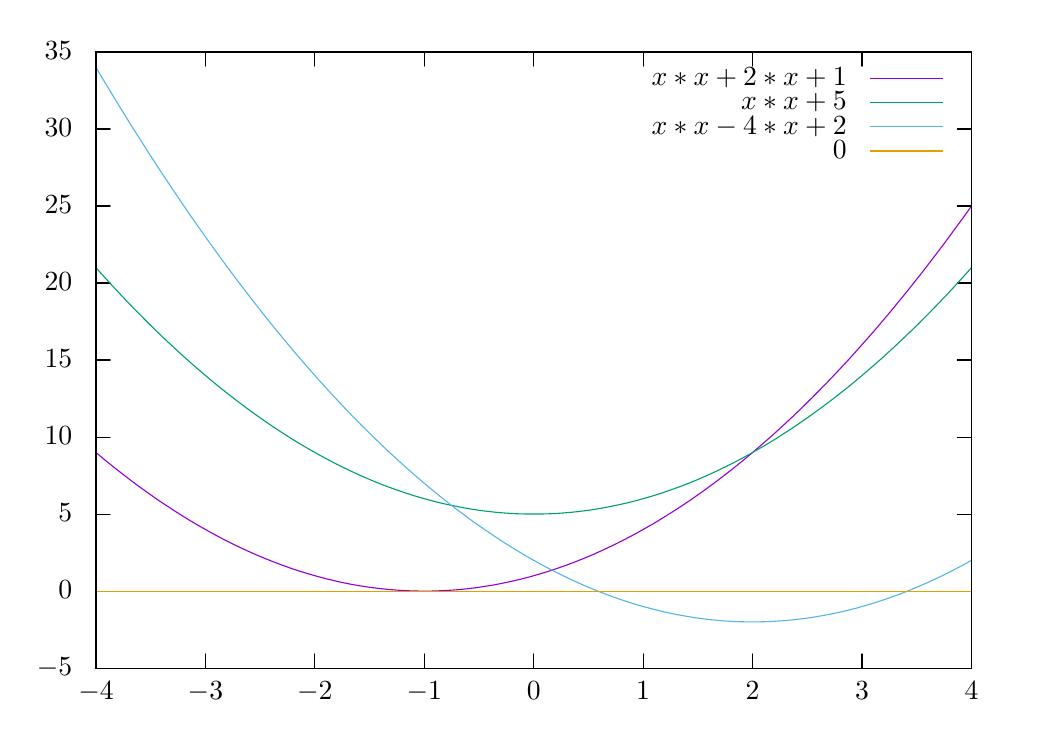
\begin{tikzpicture}[gnuplot]
%% generated with GNUPLOT 5.4p2 (Lua 5.4; terminal rev. Jun 2020, script rev. 114)
%% 2022年07月03日 星期日 22时58分01秒
\path (0.000,0.000) rectangle (12.500,8.750);
\gpcolor{color=gp lt color border}
\gpsetlinetype{gp lt border}
\gpsetdashtype{gp dt solid}
\gpsetlinewidth{1.00}
\draw[gp path] (0.828,0.616)--(1.008,0.616);
\draw[gp path] (11.947,0.616)--(11.767,0.616);
\node[gp node right] at (0.644,0.616) {$-5$};
\draw[gp path] (0.828,1.594)--(1.008,1.594);
\draw[gp path] (11.947,1.594)--(11.767,1.594);
\node[gp node right] at (0.644,1.594) {$0$};
\draw[gp path] (0.828,2.572)--(1.008,2.572);
\draw[gp path] (11.947,2.572)--(11.767,2.572);
\node[gp node right] at (0.644,2.572) {$5$};
\draw[gp path] (0.828,3.550)--(1.008,3.550);
\draw[gp path] (11.947,3.550)--(11.767,3.550);
\node[gp node right] at (0.644,3.550) {$10$};
\draw[gp path] (0.828,4.529)--(1.008,4.529);
\draw[gp path] (11.947,4.529)--(11.767,4.529);
\node[gp node right] at (0.644,4.529) {$15$};
\draw[gp path] (0.828,5.507)--(1.008,5.507);
\draw[gp path] (11.947,5.507)--(11.767,5.507);
\node[gp node right] at (0.644,5.507) {$20$};
\draw[gp path] (0.828,6.485)--(1.008,6.485);
\draw[gp path] (11.947,6.485)--(11.767,6.485);
\node[gp node right] at (0.644,6.485) {$25$};
\draw[gp path] (0.828,7.463)--(1.008,7.463);
\draw[gp path] (11.947,7.463)--(11.767,7.463);
\node[gp node right] at (0.644,7.463) {$30$};
\draw[gp path] (0.828,8.441)--(1.008,8.441);
\draw[gp path] (11.947,8.441)--(11.767,8.441);
\node[gp node right] at (0.644,8.441) {$35$};
\draw[gp path] (0.828,0.616)--(0.828,0.796);
\draw[gp path] (0.828,8.441)--(0.828,8.261);
\node[gp node center] at (0.828,0.308) {$-4$};
\draw[gp path] (2.218,0.616)--(2.218,0.796);
\draw[gp path] (2.218,8.441)--(2.218,8.261);
\node[gp node center] at (2.218,0.308) {$-3$};
\draw[gp path] (3.608,0.616)--(3.608,0.796);
\draw[gp path] (3.608,8.441)--(3.608,8.261);
\node[gp node center] at (3.608,0.308) {$-2$};
\draw[gp path] (4.998,0.616)--(4.998,0.796);
\draw[gp path] (4.998,8.441)--(4.998,8.261);
\node[gp node center] at (4.998,0.308) {$-1$};
\draw[gp path] (6.388,0.616)--(6.388,0.796);
\draw[gp path] (6.388,8.441)--(6.388,8.261);
\node[gp node center] at (6.388,0.308) {$0$};
\draw[gp path] (7.777,0.616)--(7.777,0.796);
\draw[gp path] (7.777,8.441)--(7.777,8.261);
\node[gp node center] at (7.777,0.308) {$1$};
\draw[gp path] (9.167,0.616)--(9.167,0.796);
\draw[gp path] (9.167,8.441)--(9.167,8.261);
\node[gp node center] at (9.167,0.308) {$2$};
\draw[gp path] (10.557,0.616)--(10.557,0.796);
\draw[gp path] (10.557,8.441)--(10.557,8.261);
\node[gp node center] at (10.557,0.308) {$3$};
\draw[gp path] (11.947,0.616)--(11.947,0.796);
\draw[gp path] (11.947,8.441)--(11.947,8.261);
\node[gp node center] at (11.947,0.308) {$4$};
\draw[gp path] (0.828,8.441)--(0.828,0.616)--(11.947,0.616)--(11.947,8.441)--cycle;
\node[gp node right] at (10.479,8.107) {$x*x + 2*x +1$};
\gpcolor{rgb color={0.580,0.000,0.827}}
\draw[gp path] (10.663,8.107)--(11.579,8.107);
\draw[gp path] (0.828,3.355)--(0.940,3.261)--(1.053,3.170)--(1.165,3.082)--(1.277,2.996)%
  --(1.390,2.912)--(1.502,2.832)--(1.614,2.753)--(1.727,2.678)--(1.839,2.605)--(1.951,2.534)%
  --(2.063,2.466)--(2.176,2.401)--(2.288,2.338)--(2.400,2.277)--(2.513,2.219)--(2.625,2.164)%
  --(2.737,2.112)--(2.850,2.061)--(2.962,2.014)--(3.074,1.969)--(3.187,1.926)--(3.299,1.886)%
  --(3.411,1.849)--(3.524,1.814)--(3.636,1.782)--(3.748,1.752)--(3.860,1.725)--(3.973,1.700)%
  --(4.085,1.678)--(4.197,1.659)--(4.310,1.642)--(4.422,1.628)--(4.534,1.616)--(4.647,1.607)%
  --(4.759,1.600)--(4.871,1.596)--(4.984,1.594)--(5.096,1.595)--(5.208,1.599)--(5.321,1.605)%
  --(5.433,1.613)--(5.545,1.624)--(5.657,1.638)--(5.770,1.655)--(5.882,1.673)--(5.994,1.695)%
  --(6.107,1.719)--(6.219,1.745)--(6.331,1.774)--(6.444,1.806)--(6.556,1.840)--(6.668,1.877)%
  --(6.781,1.916)--(6.893,1.958)--(7.005,2.002)--(7.118,2.049)--(7.230,2.099)--(7.342,2.151)%
  --(7.454,2.205)--(7.567,2.263)--(7.679,2.322)--(7.791,2.385)--(7.904,2.449)--(8.016,2.517)%
  --(8.128,2.587)--(8.241,2.659)--(8.353,2.734)--(8.465,2.812)--(8.578,2.892)--(8.690,2.975)%
  --(8.802,3.060)--(8.915,3.148)--(9.027,3.238)--(9.139,3.331)--(9.251,3.427)--(9.364,3.525)%
  --(9.476,3.625)--(9.588,3.728)--(9.701,3.834)--(9.813,3.942)--(9.925,4.053)--(10.038,4.167)%
  --(10.150,4.282)--(10.262,4.401)--(10.375,4.522)--(10.487,4.646)--(10.599,4.772)--(10.712,4.900)%
  --(10.824,5.032)--(10.936,5.165)--(11.048,5.302)--(11.161,5.441)--(11.273,5.582)--(11.385,5.726)%
  --(11.498,5.873)--(11.610,6.022)--(11.722,6.174)--(11.835,6.328)--(11.947,6.485);
\gpcolor{color=gp lt color border}
\node[gp node right] at (10.479,7.799) {$x*x+5$};
\gpcolor{rgb color={0.000,0.620,0.451}}
\draw[gp path] (10.663,7.799)--(11.579,7.799);
\draw[gp path] (0.828,5.702)--(0.940,5.577)--(1.053,5.454)--(1.165,5.334)--(1.277,5.217)%
  --(1.390,5.102)--(1.502,4.989)--(1.614,4.880)--(1.727,4.772)--(1.839,4.668)--(1.951,4.565)%
  --(2.063,4.466)--(2.176,4.369)--(2.288,4.274)--(2.400,4.182)--(2.513,4.093)--(2.625,4.006)%
  --(2.737,3.922)--(2.850,3.840)--(2.962,3.761)--(3.074,3.684)--(3.187,3.610)--(3.299,3.538)%
  --(3.411,3.469)--(3.524,3.403)--(3.636,3.339)--(3.748,3.278)--(3.860,3.219)--(3.973,3.163)%
  --(4.085,3.109)--(4.197,3.058)--(4.310,3.009)--(4.422,2.963)--(4.534,2.920)--(4.647,2.879)%
  --(4.759,2.841)--(4.871,2.805)--(4.984,2.772)--(5.096,2.741)--(5.208,2.713)--(5.321,2.688)%
  --(5.433,2.665)--(5.545,2.644)--(5.657,2.626)--(5.770,2.611)--(5.882,2.598)--(5.994,2.588)%
  --(6.107,2.580)--(6.219,2.575)--(6.331,2.573)--(6.444,2.573)--(6.556,2.575)--(6.668,2.580)%
  --(6.781,2.588)--(6.893,2.598)--(7.005,2.611)--(7.118,2.626)--(7.230,2.644)--(7.342,2.665)%
  --(7.454,2.688)--(7.567,2.713)--(7.679,2.741)--(7.791,2.772)--(7.904,2.805)--(8.016,2.841)%
  --(8.128,2.879)--(8.241,2.920)--(8.353,2.963)--(8.465,3.009)--(8.578,3.058)--(8.690,3.109)%
  --(8.802,3.163)--(8.915,3.219)--(9.027,3.278)--(9.139,3.339)--(9.251,3.403)--(9.364,3.469)%
  --(9.476,3.538)--(9.588,3.610)--(9.701,3.684)--(9.813,3.761)--(9.925,3.840)--(10.038,3.922)%
  --(10.150,4.006)--(10.262,4.093)--(10.375,4.182)--(10.487,4.274)--(10.599,4.369)--(10.712,4.466)%
  --(10.824,4.565)--(10.936,4.668)--(11.048,4.772)--(11.161,4.880)--(11.273,4.989)--(11.385,5.102)%
  --(11.498,5.217)--(11.610,5.334)--(11.722,5.454)--(11.835,5.577)--(11.947,5.702);
\gpcolor{color=gp lt color border}
\node[gp node right] at (10.479,7.491) {$x*x-4*x+2$};
\gpcolor{rgb color={0.337,0.706,0.914}}
\draw[gp path] (10.663,7.491)--(11.579,7.491);
\draw[gp path] (0.828,8.245)--(0.940,8.057)--(1.053,7.871)--(1.165,7.688)--(1.277,7.507)%
  --(1.390,7.329)--(1.502,7.153)--(1.614,6.980)--(1.727,6.810)--(1.839,6.642)--(1.951,6.476)%
  --(2.063,6.313)--(2.176,6.153)--(2.288,5.995)--(2.400,5.840)--(2.513,5.687)--(2.625,5.537)%
  --(2.737,5.390)--(2.850,5.245)--(2.962,5.102)--(3.074,4.962)--(3.187,4.825)--(3.299,4.690)%
  --(3.411,4.558)--(3.524,4.428)--(3.636,4.301)--(3.748,4.177)--(3.860,4.055)--(3.973,3.935)%
  --(4.085,3.818)--(4.197,3.704)--(4.310,3.592)--(4.422,3.483)--(4.534,3.376)--(4.647,3.272)%
  --(4.759,3.171)--(4.871,3.072)--(4.984,2.975)--(5.096,2.881)--(5.208,2.790)--(5.321,2.701)%
  --(5.433,2.615)--(5.545,2.531)--(5.657,2.450)--(5.770,2.372)--(5.882,2.296)--(5.994,2.222)%
  --(6.107,2.151)--(6.219,2.083)--(6.331,2.017)--(6.444,1.954)--(6.556,1.893)--(6.668,1.835)%
  --(6.781,1.780)--(6.893,1.727)--(7.005,1.676)--(7.118,1.628)--(7.230,1.583)--(7.342,1.540)%
  --(7.454,1.500)--(7.567,1.462)--(7.679,1.427)--(7.791,1.395)--(7.904,1.365)--(8.016,1.337)%
  --(8.128,1.312)--(8.241,1.290)--(8.353,1.270)--(8.465,1.253)--(8.578,1.238)--(8.690,1.226)%
  --(8.802,1.216)--(8.915,1.209)--(9.027,1.205)--(9.139,1.203)--(9.251,1.204)--(9.364,1.207)%
  --(9.476,1.213)--(9.588,1.221)--(9.701,1.232)--(9.813,1.245)--(9.925,1.261)--(10.038,1.280)%
  --(10.150,1.301)--(10.262,1.324)--(10.375,1.350)--(10.487,1.379)--(10.599,1.411)--(10.712,1.444)%
  --(10.824,1.481)--(10.936,1.520)--(11.048,1.561)--(11.161,1.605)--(11.273,1.652)--(11.385,1.701)%
  --(11.498,1.753)--(11.610,1.807)--(11.722,1.864)--(11.835,1.923)--(11.947,1.985);
\gpcolor{color=gp lt color border}
\node[gp node right] at (10.479,7.183) {$0$};
\gpcolor{rgb color={0.902,0.624,0.000}}
\draw[gp path] (10.663,7.183)--(11.579,7.183);
\draw[gp path] (0.828,1.594)--(0.940,1.594)--(1.053,1.594)--(1.165,1.594)--(1.277,1.594)%
  --(1.390,1.594)--(1.502,1.594)--(1.614,1.594)--(1.727,1.594)--(1.839,1.594)--(1.951,1.594)%
  --(2.063,1.594)--(2.176,1.594)--(2.288,1.594)--(2.400,1.594)--(2.513,1.594)--(2.625,1.594)%
  --(2.737,1.594)--(2.850,1.594)--(2.962,1.594)--(3.074,1.594)--(3.187,1.594)--(3.299,1.594)%
  --(3.411,1.594)--(3.524,1.594)--(3.636,1.594)--(3.748,1.594)--(3.860,1.594)--(3.973,1.594)%
  --(4.085,1.594)--(4.197,1.594)--(4.310,1.594)--(4.422,1.594)--(4.534,1.594)--(4.647,1.594)%
  --(4.759,1.594)--(4.871,1.594)--(4.984,1.594)--(5.096,1.594)--(5.208,1.594)--(5.321,1.594)%
  --(5.433,1.594)--(5.545,1.594)--(5.657,1.594)--(5.770,1.594)--(5.882,1.594)--(5.994,1.594)%
  --(6.107,1.594)--(6.219,1.594)--(6.331,1.594)--(6.444,1.594)--(6.556,1.594)--(6.668,1.594)%
  --(6.781,1.594)--(6.893,1.594)--(7.005,1.594)--(7.118,1.594)--(7.230,1.594)--(7.342,1.594)%
  --(7.454,1.594)--(7.567,1.594)--(7.679,1.594)--(7.791,1.594)--(7.904,1.594)--(8.016,1.594)%
  --(8.128,1.594)--(8.241,1.594)--(8.353,1.594)--(8.465,1.594)--(8.578,1.594)--(8.690,1.594)%
  --(8.802,1.594)--(8.915,1.594)--(9.027,1.594)--(9.139,1.594)--(9.251,1.594)--(9.364,1.594)%
  --(9.476,1.594)--(9.588,1.594)--(9.701,1.594)--(9.813,1.594)--(9.925,1.594)--(10.038,1.594)%
  --(10.150,1.594)--(10.262,1.594)--(10.375,1.594)--(10.487,1.594)--(10.599,1.594)--(10.712,1.594)%
  --(10.824,1.594)--(10.936,1.594)--(11.048,1.594)--(11.161,1.594)--(11.273,1.594)--(11.385,1.594)%
  --(11.498,1.594)--(11.610,1.594)--(11.722,1.594)--(11.835,1.594)--(11.947,1.594);
\gpcolor{color=gp lt color border}
\draw[gp path] (0.828,8.441)--(0.828,0.616)--(11.947,0.616)--(11.947,8.441)--cycle;
%% coordinates of the plot area
\gpdefrectangularnode{gp plot 1}{\pgfpoint{0.828cm}{0.616cm}}{\pgfpoint{11.947cm}{8.441cm}}
\end{tikzpicture}
%% gnuplot variables

  \caption{$\Delta$的三种取值情况所对应的根及其个数}
\end{figure}

\end{document}
